\documentclass[12pt,twoside]{extarticle}
\usepackage{extsizes}
\usepackage[paperheight=37.5cm,paperwidth=31.75cm, top=3.875cm,bottom=5.425cm,right=4.65cm,left=3.1cm]{geometry}
\usepackage[export]{adjustbox}
\usepackage{amsmath}
\usepackage{amsthm}
\usepackage{graphicx}
\usepackage{xcolor}
\usepackage{hyperref}
\usepackage{booktabs}
\usepackage{unicode-math}
%\unimathsetup{math-style=ISO, partial=upright, nabla=upright}
\setmainfont[Numbers=Tabular]{ScalaOT}
\setmathfont{Stix2Math.otf}
\setmathfont[range=it]{ScalaOT-Italic}
\setmathfont[range=\mathup/{num},Numbers={Tabular,Lining}]{ScalaOT}
%\setmathfont[range={"0030-"0039}]{ScalaOT}
\setmathfont[range=\mathup/{greek,Greek}]{Alegreya-Regular.otf}
\setmathfont[range=\mathit/{greek,Greek}]{Alegreya-Regular.otf}
\setmathfont[range={"002C}]{ScalaOT}
\setmathfont[range="002A]{ScalaOT}
\setmathfont[range={"222B},Scale=1.15]{LIBERTINUSMATH-REGULAR.otf}
\setsansfont[Numbers=Tabular]{SCALASANSPRO-REGULAR.otf}
\newfontfamily\myfontA[Numbers={Tabular,OldStyle}]{BEMBOBOOKMTSTD-REGULAR.otf}
\newfontfamily\myfontB[Numbers={Tabular,OldStyle}]{SCALASANSPRO-ITALIC.otf}
\newfontface\myfontC[]{AlegreyaSans-Regular.otf}
\definecolor{myblue}{RGB}{11, 79, 160}
\setlength{\footskip}{70pt}

\usepackage{listings} %For code in appendix
\lstset
{ %Formatting for code in appendix
    language=R,
    basicstyle=\footnotesize,
    numbers=left,
    stepnumber=1,
    showstringspaces=false,
    tabsize=1,
    breaklines=true,
    breakatwhitespace=false,
}

\begin{document}
\noindent 
 \begin{minipage}[t]{0.5\textwidth}
This seems like a pretty famous graph\footnotemark.  Let's try to draw it.
\end{minipage}\hfill
\footnotetext{\textsf{Credited to:  Tufte, Edward R. }\myfontB{The Visual Display of Quantitative Information}\textsf{.  But it looks like an attempt at a corrected version, because it differs from the one in the book.  I downloaded it from }\texttt{\url{https://www.edwardtufte.com/bboard/q-and-a-fetch-msg?msg_id=0003nk}}\textsf{ on May 12, 2019.}}
\adjustbox{valign=t}{\begin{minipage}[]{1\textwidth}
\vspace{2em} \raggedleft \includegraphics[]{TufteOrig.png}
\end{minipage}}%
\newpage
\noindent
\adjustbox{valign=t}{\begin{minipage}[12cm]{0.42\textwidth}
\raggedright
\vspace{1em}
\begin{myfontA}
\bgroup
\def\arraystretch{1.25}%
\begin{tabular*}{7.5cm}%
{@{\extracolsep{\fill}}lrr@{}} \toprule
Country & 1970 & 1979 \\ \midrule
Sweden & 46.9 & 57.4 \\ 
Netherlands & 44.0 & 55.8 \\ 
Norway & 43.5 & 52.2 \\ 
Britain & 40.7 & 39.0 \\ 
France & 39.0 & 43.4 \\ 
Germany & 37.5 & 42.9 \\ 
Belgium & 35.2 & 43.2 \\ 
Canada & 35.2 & 35.8 \\ 
Finland & 34.9 & 38.2 \\ 
Italy & 30.4 & 35.7 \\
United States & 30.3 & 32.5 \\ 
Greece & 26.8 & 30.6 \\ 
Switzerland & 26.5 & 33.2 \\ 
Spain & 22.5 & 27.1 \\ 
Japan & 20.7 & 26.6 \\ 
\end{tabular*}
\egroup
\end{myfontA}
\end{minipage}}%
\hfill
\adjustbox{valign=t}{\begin{minipage}[12cm]{.53\textwidth}
\section{Drawing the Slopegraph}
Given two labeled columns of numbers, we begin by drawing on the usual Cartesian plane.  Each label's line is derived from two points, ($x_1$, $c_1$) and ($x_2$, $c_2$).  $x_1$ is the value from Column 1, $x_2$ is the value from Column 2.  $c_1$ and $c_2$ are the same for each line.  The parameter $c_2-c_1$ will determine the width of the final graph.  It can be changed by the constructor to adjust the aspect ratio.  The plane is rotated clockwise $90$° and flipped and a second set of labels is added.  $c_2-c_1$ now determines the $x$-axis.  We only need to ensure consistent spacing on the new $y$-axis to produce accurate slopes.  
\end{minipage}}
\adjustbox{valign=t}{\begin{minipage}[]{1\textwidth}
\vspace{1em} \raggedleft \includegraphics[]{TufteDraw13.eps}
\end{minipage}}%
\newpage
\noindent
\adjustbox{valign=t}{\begin{minipage}[28.2cm]{0.53\textwidth}
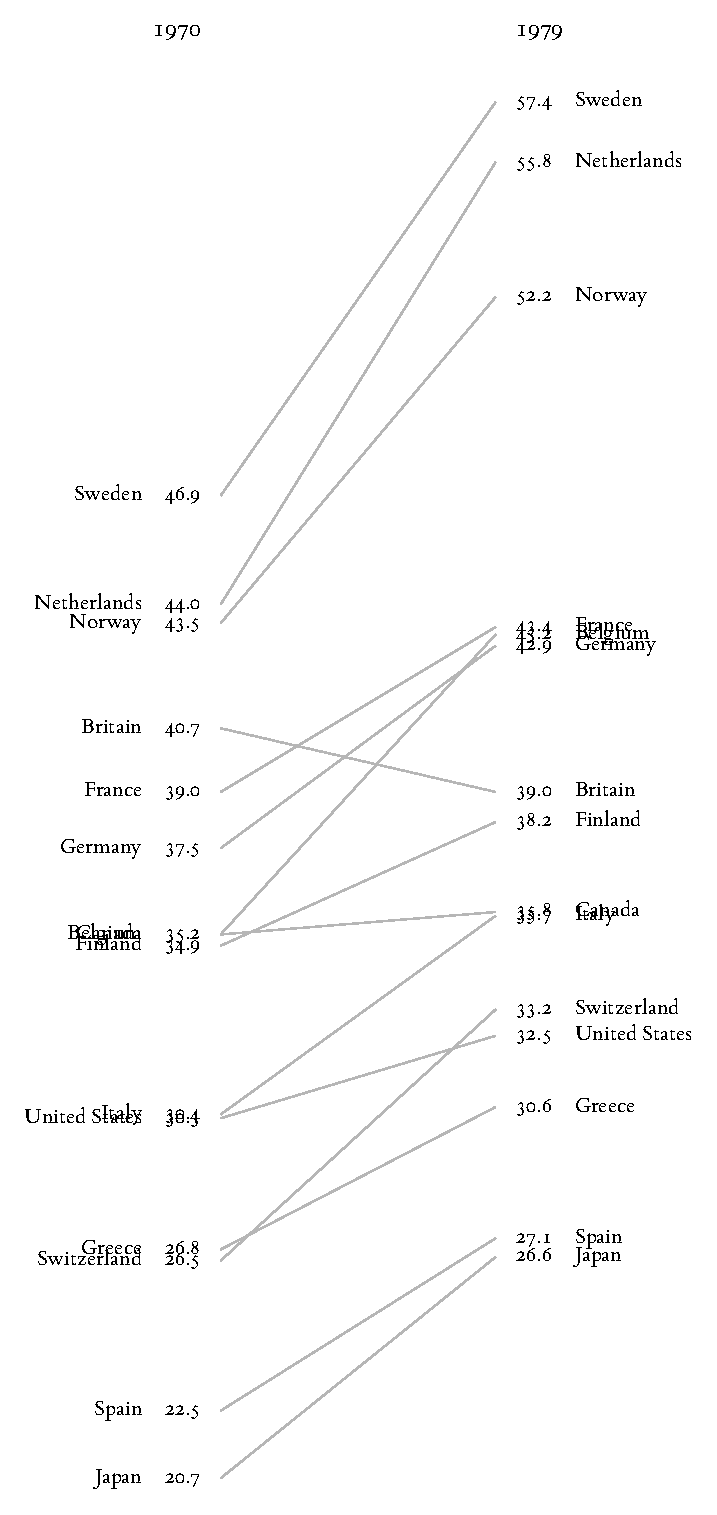
\includegraphics[]{TufteCrash.eps}
\end{minipage}}%
\hfill
\adjustbox{valign=t}{\begin{minipage}[t][28.2cm][t]{0.02\textwidth}
\vline height 28.2cm  width 1pt
\end{minipage}}
\hfill
\adjustbox{valign=t}{\begin{minipage}[t]{0.42\textwidth}
\section{ A First Attempt}
We'll plot using D3.js.  Tufte’s graph seems to be dropping $\approx$$24$ pixels for every $1$ percentage point in GDP, so that’s what we’ll use for our \textbf{\emph{drop coefficient}} ($\delta$).  We put the top point, Sweden[57.4], at position $0$, and every other point's position is determined by its distance from $57.4$ times $24$.  E.g., for Norway:  
\begin{align*}
y_{Norway,1} &= (57.4-43.5)\cdot 24=333.6 \\
y_{Norway,2} &= (57.4-52.2)\cdot24=124.8
\end{align*}
Higher $y$-values move us further down the page because D3.js’s $y$-axis is upside-down. The drop coefficient is chosen to translate the scale of the data into something that will (eventually) fit on the screen.  Here, the maximum element is $57.4$, the minimum is $20.7$, the difference is $57.4-20.7=36.7$. If we let $1$ unit of the data equal $24$ pixels, our graph will be a little over $36.7 \cdot 24 \approx 881$ pixels long, which should be okay for a typical screen.\par
\vspace{1em}
The result is shown to the left.  Obviously, some points are too close together to get proper spacing for their labels.  There may be many ways to fix these crashed labels, and what's best will depend upon the situation.  My solution is to frame it as a constrained optimization problem.  I can minimize the difference between the points and where they should be, subject to the constraints that the lines have the same drop coefficient, and that there's a minimum distance between all points in each column.\par
\vspace{1em}
The problem I’ve developed is a straightforward quadratic programming problem (quadratic objective function, linear constraints), so there are many optimizers that can handle it.  I’m using the “alabama” solver in R with the ROI package as an interface.  My code will import a .csv file; construct an objective function, constraints, and a staring point within the problem's feasible region; solve the problem; output points ready to be copied and pasted into a D3.js thing; check that $\delta$ is (nearly) the same for each line.\par
\vspace{1em}
The program, as I’ve written it, expects the first column of the data to be in order.  If there are ties, the order in which the tied points are presented could dramatically affect the outcome of the graph, so I’ve left the sorting decisions to the user.  Our first task will be to develop a set of ideal points, to… The ideal points will be the points I just plotted (they're in the correct positions, after all), with adjustments made for the ties.
\end{minipage}}
\newpage 
\noindent
\adjustbox{valign=t}{\begin{minipage}[t][]{0.42\textwidth}
\section{Optimization}
For the general case, where we have $n$ rows of two labelled columns of numbers, 
\begin{align*}
	\left \{x_{1j},\dots ,x_{nj} \right \} :=  \quad \text{The numbers in column } j \text{ for } j=1,2.
\end{align*}
We establish the ideal vertical positions using our chosen drop coefficient, $\delta$.  The positions are adjusted slightly so that no two are the same within the same column.
\begin{align*}
y_{ij}^* = \delta(\max_{i,j}(x_{ij})-x_{ij})
\end{align*}
Call the minimum distance between any two nontied points in either column $d$,
\begin{align*}
d = \min(\lvert y_{kj}^*-y_{ij}^*\rvert : y_{kj}^* \neq y_{ij}^*)
\end{align*}
For any $x_{ij}$ that is duplicated, collect each of the duplicates into a set, $V_{x_{ij}}$.
\begin{align*}
x_{kj} \in V_{x_{ij}} \qquad &\text{ if } x_{kj}=x_{ij} \text{ and } k>i \\
V_{x_{ij}} = \emptyset \qquad &\text{ if } x_{kj} \neq x_{ij} \text{ for } k \neq i
\end{align*}
Let $m_j = \max(\lvert V_{x_{ij}} \rvert)$ be the number of elements in the $V_{x_{ij}}$ with the greatest cardinality for each column, $j$.  Index each $V_{x_{ij}}$ with $v_{ijk}$, the rank (in ascending order) of $k$ among the row indices of the $m$ points in $V_{x_{ij}}$,

\begin{align*}
v_{ij1} &= \min(k:x_{kj} \in V_{x_{ij}}) \\
v_{ij2} &= \min(k:x_{kj} \in V_{x_{ij}}\setminus \left \{x_{v_{ij1}j} \right \}) \\
&\vdots \\
v_{ijm} &= \max(k:x_{kj} \in V_{x_{ij}})
\end{align*}

First, we make new assignments to the points in Column 1:
\begin{align*}
\text{For every } x_{k1} \in V_{x_{i1}}, \\
y_{kj}^* := y_{kj}^* + v_{i1k}(\frac{d}{m_1+1})
\end{align*}
Then, for Column 2:
\vspace{1em}
\newline
For every $x_{k2} \in V_{x_{i2}}$,
\begin{align*}
y_{kj}^* := y_{kj}^* + v_{i2k}(\frac{d}{(m_1+1)(m_2+1)})
\end{align*}

Now that all of the necessary $y_{ij}^*$ have been adjusted, we are ready to declare them to be our $\left \{ y_{ij} \right \}_{\substack{1 \leq i \leq n \\ j=1,2}}$, the set of ideal vertical positions to which we aspire.

\begin{align*}
y_{ij} := y_{ij}^* \quad &\text{for }1 \leq i \leq n, j = 1,2.
\end{align*}

%$\left \{y_{1j},\dots ,y_{nj} \right \} := \quad \text{The ideal positions of the } x_{ij} \text{ (if there were no concerns about crashed labels)}$
%$\left \{\hat{y}_{1j},\dots ,\hat{y}_{nj} \right \}  := \quad \text{The fitted positions of the }x_{ij}$
\end{minipage}}%
\hspace{1.2cm} 
\adjustbox{valign=t}{\begin{minipage}[t]{0.53\textwidth}
The function to be optimized (minimized) is the sum of squared distances between the fitted points,$\hat{y}_{ij}$, and their ideal placements,$y_{ij}$.  The \textbf{objective function} is:

\begin{align*}
\sum_{j=1}^{2}\sum_{i=1}^{n}(y_{ij}-\hat{y}_{ij})^2
\end{align*}

The first constraint keeps the drop coefficients the same, within some tolerance.  Let {\myfontC є} $>0$ be some small number.  \textbf{Constraint 1:}
\begin{align*}
-\text{\myfontC є} \leq \frac{\hat{y}_{i,1}-\hat{y}_{i,2}}{x_{i,1}-x_{i,2}}\ - \frac{\hat{y}_{k1}-\hat{y}_{k2}}{x_{k1}-x_{k2}}\ &\leq \text{\myfontC є} \\
\text{for all } i,k \text{ such that }x_{i1}-x_{i,2} \neq 0 \text{ and } x_{k,1}-x_{k,2} \neq 0 \\
\hat{y}_{i1}-\hat{y}_{i2} &=0 
\text{for all } i \text{ such that } x_{i1}-x_{i2} = 0
\end{align*}

\textbf{Constraint 2} will make sure that the points stay in order, and that the minimum distance between them is $\zeta$ pixels, where $\zeta$ is chosen to provide the appropriate line spacing (I'm using $\zeta=16$ for an $11.5$ pt. font):

\begin{align*}
\hat{y}_{kj}-\hat{y}_{ij} \geq \zeta \quad \text{ for all }i,j,k \text{ such that }y_{kj} > y_{ij} 
\end{align*}

Besides the first and last, every number in a column is sandwiched in between two other numbers.  We can make a constraint that puts the label closer to whichever number is closer.  E.g., we can place Germany[37.5] closer to France[39.0] than to Belgium[35.2], since $39.0-37.5 < 37.5-35.2$.  \textbf{Constraint 3:}

\begin{align*}
\text{For }k \text{ satisfying }\min_{1 \leq i \leq n}{(y_{i1})} < y_{k1} < \max_{1 \leq i \leq n}(y_{i1}), \\
\text{Let } u \text{ be such that }  y_{u1} = \min(\left \{y_{i1} : x_{i1} \leq x_{k1}, i \neq k \right \}) \\
\text{Let } l \text{ be such that }  y_{l1} = \max(\left \{y_{i1} : x_{i1} \geq x_{k1}, i\neq k \right \}) \\
\text{Then, } \\
x_{i1}-x_{u1} > x_{l1}-x_{i1} \implies \hat{y}_{u1} + \hat{y}_{l1} - 2\hat{y}_{i1} \geq 0, \\
x_{i1}-x_{u1} < x_{l1}-x_{i1} \implies 2\hat{y}_{i1} - \hat{y}_{u1} - \hat{y}_{l1}  \geq 0
\end{align*}

\textbf{Constraint 4} is the same as Constraint 3, except that it applies to Column 2. 


Other constraints could be added, but they'd reduce the number of potential solutions.  I wasn't able to get a graph on a scale close to Tufte's using all four constraints.  My graph is drawn under Constraints 1, 2, and 4. 
\end{minipage}}
\newpage
\noindent
\begin{minipage}[]{1\textwidth}
\section{Comparisons}
Tufte's graph, side-by-side with \textcolor{myblue}{mine}:  the Sweden[57.4]'s are aligned as perfectly as I could get them.  I can tell right away that some of the slopes are different.  On my graph, there's no way to get Finland[38.2] as close to Britain[39.0] as Tufte has it, because moving up Finland sets off a chain reaction that moves up Britain...
\end{minipage}%
\hfill
\vspace{1.5em}
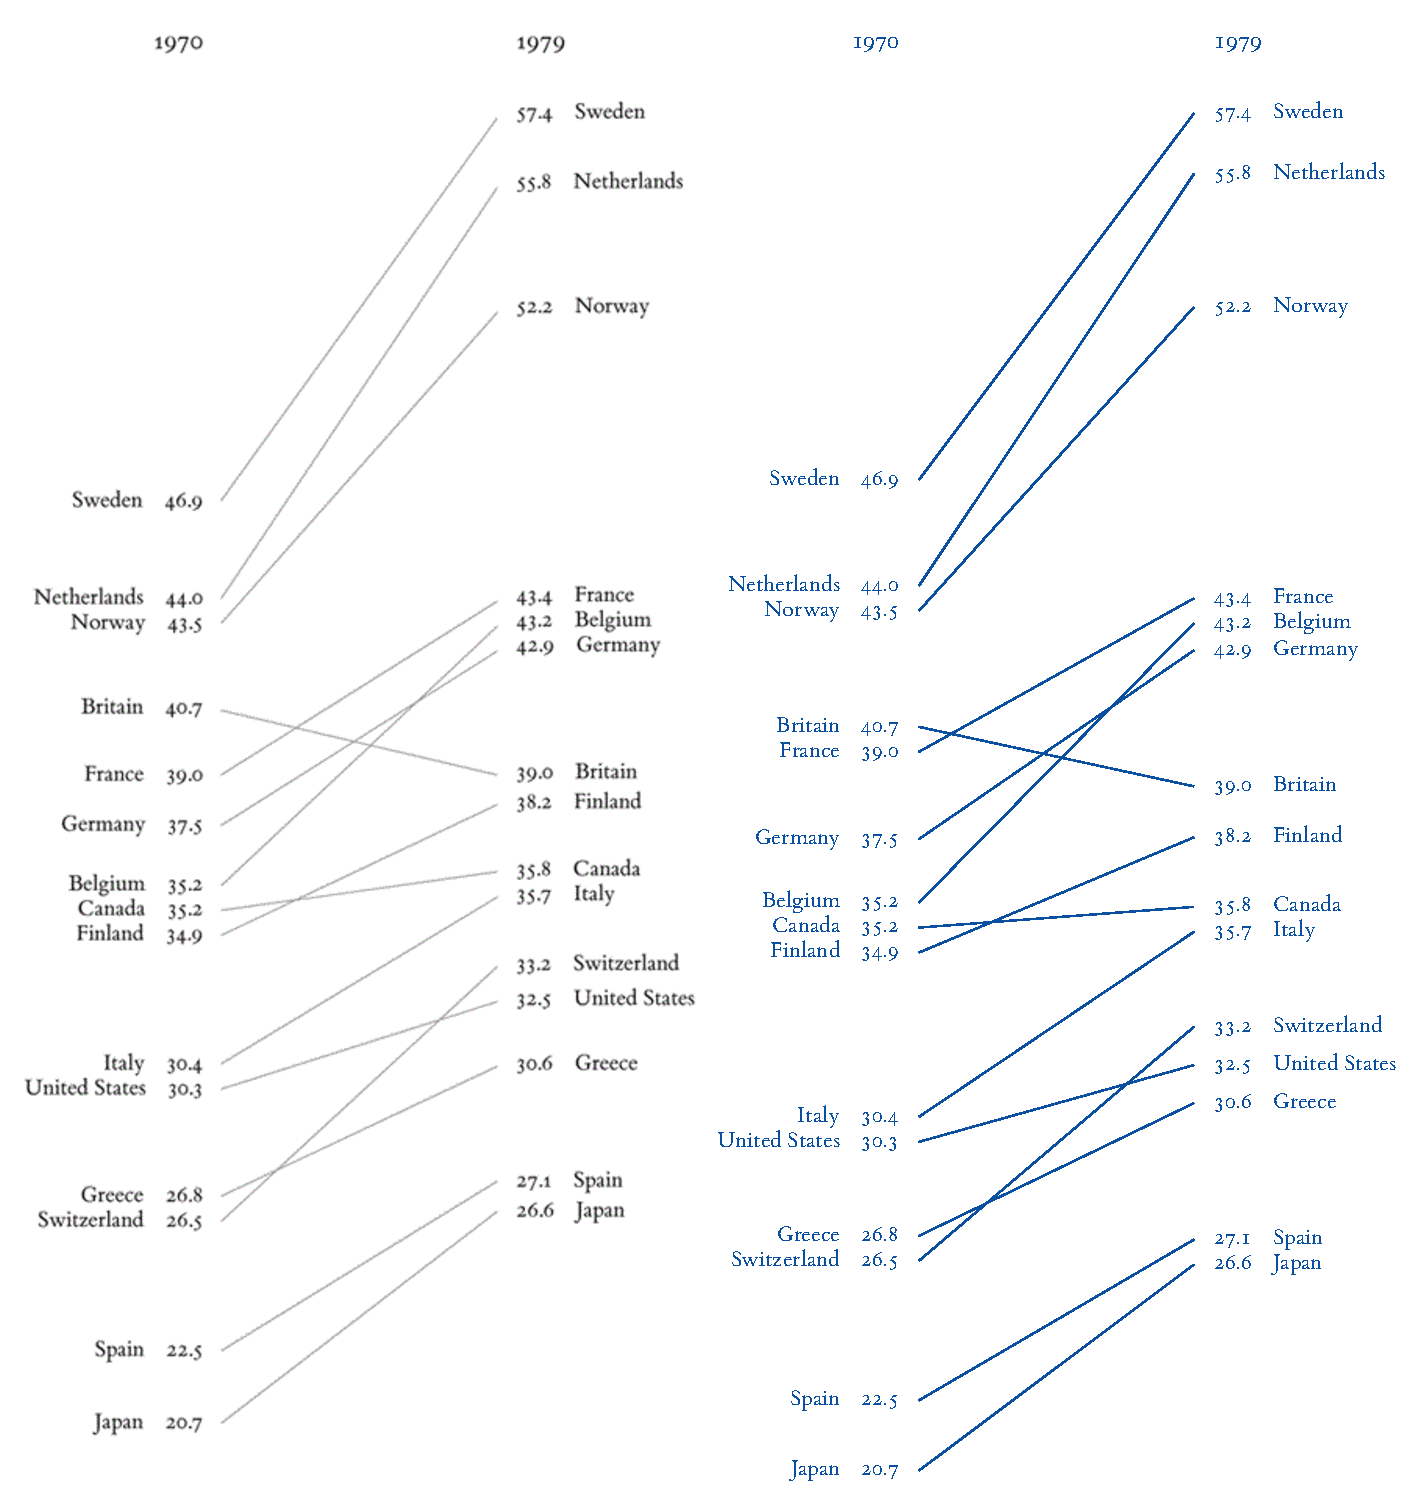
\includegraphics[]{TuftesVsMineSBS.eps}
\newpage
\noindent
\adjustbox{valign=t}{\begin{minipage}[]{0.42\textwidth}
From the overlay, we can see the degrees to which my lines agree with his.  There's a check at the end of my code, so I know that mine are correct.  The slopes are obviously the most important part of this visualization.  We don't \emph{need} the scales of the two axes to be perfectly accurate--in fact we expect them to be somewhat off whenever there are crashes.  If the scales are too bad, then we'll have an ugly graph, but I don't think that justifies distorting the slopes. \par
\vspace{1em}
A clue to what might have happened can be found in his book.  Here's a photo of the slopegraph on pg. 158 of the 2nd edition of \emph{The Visual Display of Quantitative Information}.\par
\vspace{1em}
{\centering\includegraphics[width=0.98\textwidth]{TufteBookVersion.jpg}\vspace{1em}}
The book's lines look different from the web page's.  They remind me of the graph with the crashed labels I drew on pg. 3.  Some of the text is not centered on the lines.  If it were, I think you'd have the web version.  I think Tufte redrew the lines in the book to better align with the text, and that's why some of them are so far off.  As it turns out, I can get pretty close replicas of both graphs by removing the constraint that keeps $\delta$ the same for each label\footnotemark.
\end{minipage}}%
\hfill
\adjustbox{valign=t}{\begin{minipage}{0.53\textwidth}
\includegraphics[]{TuftesVsMineOverlay60.png}
\end{minipage}}
\footnotetext{\textsf{I had to rewrite some of my code to do this.  It had never occurred to me to make this constraint optional.}}
\newpage
\noindent
\adjustbox{valign=t}{\begin{minipage}{0.475\textwidth}
1)\hspace{1em}This is my interpretation of Tufte's book version.  I used Constraint 2 to adjust the spacing of the labels, but left the lines alone.
\end{minipage}}%
\hfill
\adjustbox{valign=t}{\begin{minipage}{0.475\textwidth}
2)\hspace{1em}This is my interpretation of Tufte's web version.  I used Constraint 2 to adjust the spacing of the labels and plotted the endpoints of the lines at the labels' positions.
\end{minipage}}%
\vspace{2em}
{\centering\includegraphics[]{Tufte2Versions.eps}}
\newpage
\noindent
\adjustbox{valign=t}{\begin{minipage}{0.53\textwidth}
Finally, here's a comparison of \textcolor{myblue}{my version} of the web version with the original, side-by-side, with overlaid lines.  The spacing is still different, but there's much more consistency in how the lines deviate from each other.
\end{minipage}}%
\hfill
\vspace{3em}
{\centering\includegraphics[]{TuftesIncorrectVsMine.eps}}
\newpage
\noindent
\includegraphics[]{GoodsBasketSlopegraph2.eps}
\newpage
\noindent
\hspace{12.6cm}\adjustbox{valign=t}{\begin{minipage}[t]{0.42\textwidth}
This is a graph of UK traffic fatalities from 2000-2013 here's a bunch of shit la la la.
\end{minipage}}\par
\vspace{-2em} \includegraphics[]{UKTraffic.eps}
\end{document}
